\chapter{Non Inertial frames and Fictitious force}
\section{Non- inertial frame}
By now we were  discussing  inertial frames ,  in which Newton's second law of motion `$\boldsymbol{F}=\mathrm{ma}$'  holds true .
There are other frames of references in which Newton's law of  inertia does not hold and  are called non- inertial frames. All the accelerated and rotating frames are the non-inertial frames of reference.\\
In an accelerated frame ,  a force-free particle will seem to have an acceleration. If we do not consider the acceleration of the frame but apply Newton's laws to the motion of the force free-particle, then it will appear that a force is acting on it.
\section{Fictitious or Pseudo force (Translational.)}
\begin{figure}[H]
	\centering
	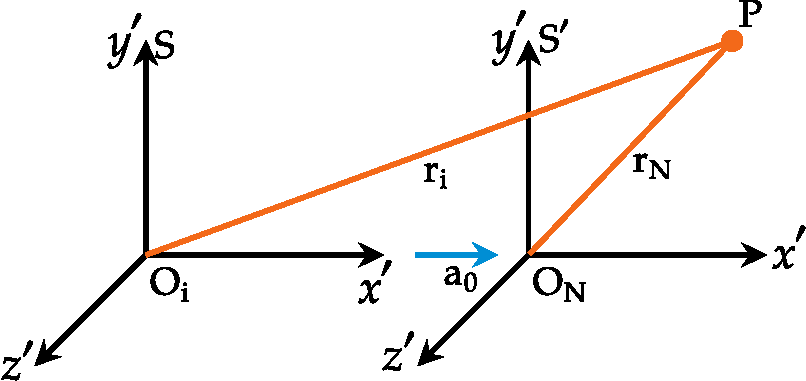
\includegraphics[height=3.5cm,width=7.5cm]{fictitious}
	\caption{}
	\label{}
\end{figure}
Let us consdier two frames $S$ and $S^{\prime}$ where, $S$ is an inertial frame and  frame $S^{\prime}$ is moving with an acceleration  $\mathrm{a}_{0}$ relative to $S$. The acceleration of a particle $P$, on which no external force is acting, will be zero in the frame $S$. But in frame $S^{\prime}$ the observer will find that an acceleration - $\mathrm{a}_{0}$ is acting on it. Thus, in frame $S^{\prime}$ the observed force on the particle is $-\mathrm{m a}_{0}$, where $m$ is the mass of the particle.  \textbf{Such a force, which does not really act on the particle but appears due to the acceleration of the frame, is called a Fictitious or pseudo force}. The fictitious force on the particle $P$ is 
\begin{equation}
\mathrm{F}_{0}=- \mathrm{m a}_{0}
\label{Ficititious 1}
\end{equation}
Hence the accelerated frame is non inertial.
If a force $\mathrm{F}_{i}$ is applied on the particle and $\mathrm{a}_{i}$ is the observed acceleration in the inertial frame $S$, then according to Newton's law
\begin{equation}
\mathrm{F}_{i}= \mathrm{ma}_{i} 
\label{Ficititious 2}
\end{equation}
Since the non inertial frame $S^{\prime}$ is moving with an acceleration  $\mathrm{a}_{0}$, We can connect the  position vectors of the two frames as,
 \begin{align}
 \mathrm{r}_{i}&=\mathrm{r}_{n}+\frac{1}{2} \mathrm{a}_{0} t^{2}\\
 \text{ Differentiating }&\text{twice we get,}\\
 \frac{d^{2} \mathrm{r}_{i}}{d t^{2}}&=\frac{d^{2} \mathrm{r}_{n}}{d t^{2}}+\mathrm{a}_{0}\\
  \frac{d^{2} \mathrm{r}_{i}}{d t^{2}}&=\mathrm{a}_{i}\quad  (\text { The acceleration in the inertial frame.}) \notag\\ \frac{d^{2} \mathrm{r}_{n}}{d t^{2}}&=\mathrm{a}_{n} \quad (\text { The acceleration observed in the non-inertial frame.}) \notag \\
  a_{i}&=a_{n}+a_{0}\notag  \\
  a_{i}-a_{0}&=a_{n} \\
  m a_{i}-m a_{0}&=m a_{n}\\
\text{And using equations }&\text{\ref{Ficititious 1} and \ref{Ficititious 2} we get}\\
  \mathrm{F}_{n}&=\mathrm{F}_{i}+\mathrm{F}_{0}
  \intertext{Thus the observer in the accelerated frame will measure the resultant (total) force which is the sum of real and fictitious forces on the particle i.e.,}
  \text{Total force}&=\text{True force} +\text{Fictitious force}
 \end{align}
 \subsection{ Free fall of a body inside a box}
 Suppose that a box is falling in the gravitational field of the earth with an acceleration $\mathrm{a}_{0}=-\mathrm{g} \hat{\mathrm{n}}$, where $g$ is the acceleration due to gravity and $\hat{n}$ is a unit vector in the upward direction. Now, if we consider a particle, falling freely inside the box, the fictitious force on the particle is $\mathrm{F}_{0}=-m \mathrm{a}_{0}=m g \hat{n}$. As the real force on the particle due to the attraction of the earth is $-m g \hat{\mathrm{n}}$, the force observed by the observer inside the box is
 \begin{equation}
 \mathrm{F}_{n}=\mathrm{F}_{i}+\mathrm{F}_{0}=-m g \hat{\mathrm{n}}+m g \hat{\mathrm{n}}=0
 \end{equation}
\textbf{ Case-1:}$\quad$ If the particle has no initial velocity relative to the box, it will seem to remain suspended in mid-air at the same place inside the box.\\\\
\textbf{ Case-2:}$\quad$ Suppose that the box is moved with an acceleration $a_{0}=g \hat{\mathrm{n}}$ in the upward direction relative to the ground. In such a case, the real force $\left(F_{i}\right)$ and fictitious force $\left(F_{0}\right)$ on the particle are given by,
\begin{equation}
 \mathrm{F}_{i}=-m g \hat{\mathrm{n}}\quad ; \quad \mathrm{F}_{0}=-m {\mathrm{a}}_{0}=-m g \hat{\mathrm{n}}
\end{equation}
Then, the total force in the accelerated frame (box) is
\begin{equation}
 \mathrm{F}_{n}=\mathrm{F}_{i}+\mathrm{F}_{0}=-m g \hat{\mathrm{n}}-m g \hat{\mathrm{n}}=-2 m g \hat{\mathrm{n}}
\end{equation}
 This means that the observer, stationed in the box having an acceleration $g$ upward, will measure a force $2 m g$ downward on the particle.
\begin{exercise}
\textbf{The Apparent Force of Gravity:}\\
	A small weight of mass $m$ hangs from a string in an automobile which accelerates at rate $A .$ What is the static angle of the string from the vertical, and what is its tension?
\end{exercise}
\begin{figure}[H]
	\centering
	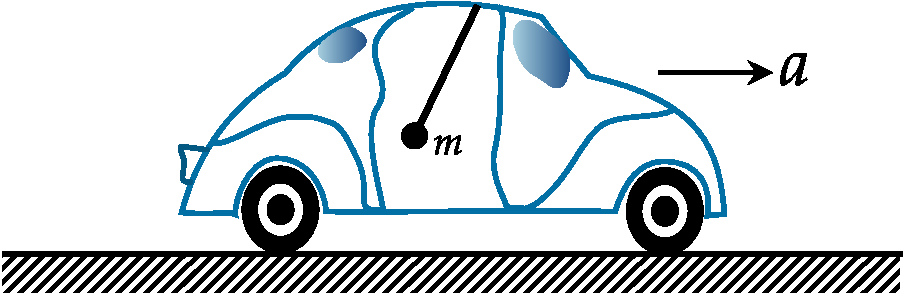
\includegraphics[height=2cm,width=7cm]{Car}
\end{figure} 
\begin{answer}
	We shall analyze the problem both in an inertial frame and in a frame accelerating with the car.\\
	\begin{minipage}{0.45\textwidth}
		$\left. \right. $\\
	$\left. \right. $ \hspace{2cm}\textbf{Inertial System}
\begin{figure}[H]
	\centering
	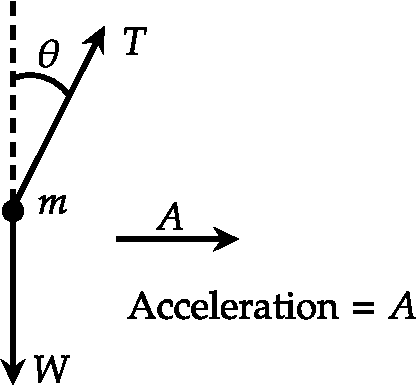
\includegraphics[height=3cm,width=4cm]{car 1}
\end{figure}
	\begin{align*}
	T \cos \theta-W &=0 \\
	T \sin \theta &=m A \\
	\tan \theta &=\frac{m A}{W}\\&=\frac{A}{g} \\
	T &=m\left(g^{2}+A^{2}\right)^{1 / 2}
	\end{align*}
	\end{minipage} \hfill
\begin{minipage}{0.45\textwidth}
		$\left. \right. $\\
\textbf{System accelerating with auto.}
\begin{figure}[H]
	\centering
	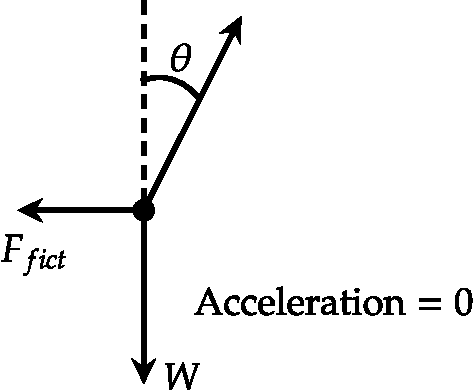
\includegraphics[height=3.5cm,width=4cm]{car2}
\end{figure}
	\begin{align*}
	T \cos \theta-W &=0 \\
	T \sin \theta-F_{\text {fict }} &=0 \\
	F_{\text {fict }} &=-m A \\
	\tan \theta &=\frac{A}{g} \\
	T &=m\left(g^{2}+A^{2}\right)^{1 / 2}
	\end{align*}
\end{minipage}\\
From the point of view of a passenger in the accelerating car, the fictitious force acts like a horizontal gravitational force. The effective gravitational force is the vector sum of the real and fictitious forces.
\end{answer}
\section{Centrifugal force}
Let us consider a mass $m$ rest in  a non -inertial frame of reference, so that in this frame, the observed acceleration or the acceleration of the particle is zero. Now suppose that a frame is rotating with an angular velocity $\vec{\omega}$ relative to an inertial frame . In this noninertial (rotating) frame, the observed acceleration $\left(\mathrm{a}_{n}\right)$ of the mass $m$ is zero.\\

\begin{minipage}{0.65\textwidth}
\begin{align*}
i.e.,\  a_{n}&=0\\
\text{ Then the total force,}\ \mathrm{F}_{n}=m \mathrm{a}_{n}&=0 \\
\mathrm{F}_{i}+\mathrm{F}_{0}&=\mathrm{F}_{n} \\
-m \vec{\omega}^{2} \mathrm{r}+\mathrm{F}_{0}&=0\\
\text{Then,}\ \mathrm{F}_{0}&=m \vec{\omega}^{2} \mathrm{r}
\intertext{This fictitious force $F_{0}$ is directed away from the centre , along $r$,   and is called the centrifugal force.}
\end{align*}
\end{minipage}\hfil
\begin{minipage}{0.25\textwidth}
	\begin{figure}[H]
		\centering
		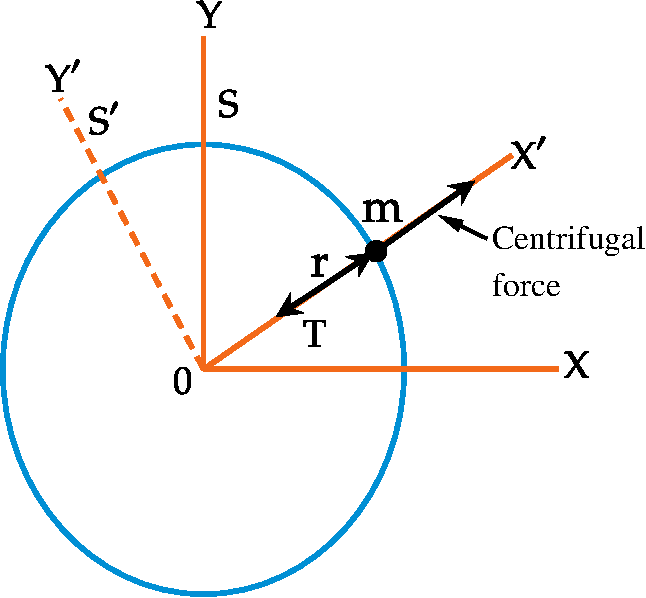
\includegraphics[height=4cm,width=4.7cm]{Centrifugal1}
		\caption{}
		\label{}
	\end{figure}
\end{minipage}\\
We know that the centrifugal force is a pseudo force and appears in the rotating frame due to its rotation . Here in the noninertial frame the centrifugal force is balanced by the inward tension in the string. In general, in the rotating frame, the centrifugal force is equal and opposite to the actual force and both are acting on the same particle. 
\section{ Uniformely Rotating Frames }
\begin{figure}[H]
	\centering
	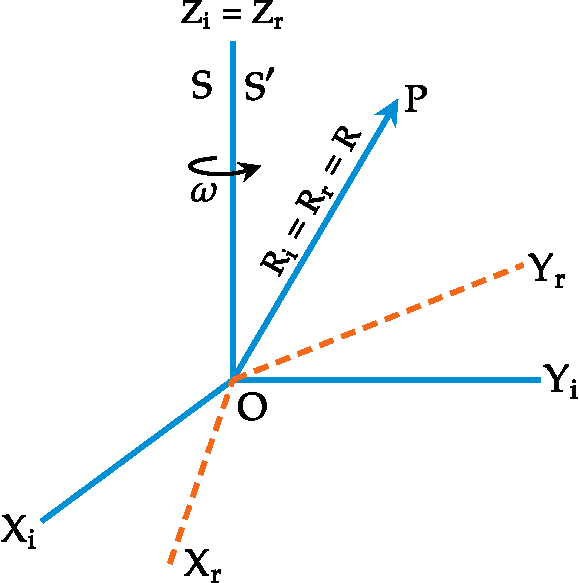
\includegraphics[height=4.2cm,width=4.2cm]{Centrifugal2}
	\caption{}
	\label{}
\end{figure}
Suppose that a frame $S^{\prime}\left(X_{r}, Y_{r}, Z_{r}\right)$ is rotating with an angular velocity $\vec{\omega}$ relative to an inertial frame $S\left(X_{i}\right.$, $\left.Y_{i}, Z_{i}\right) .$ For simplicity, we assume that both of the frames have common origin $O$ and common $Z$-axis.\\
The position vector of a particle $P$ in both frames will be the same $^{+}$, i.e., $\mathrm{R}_{i}=\mathrm{R}_{r}=\mathrm{R}$, because the origins are coincident. Now, if the particle $P$ is stationary in the frame $S$, the observer in the rotating frame $S^{\prime}$ will see that the particle is moving oppositely with linear velocity $-\vec{\omega} \times \mathrm{R}$. 
\begin{align}
\text { If the velocity of the }&\text{particle in the frame $S$,}\\
v_{i} &=\left(\frac{d \mathrm{R}}{d t}\right)_{i}\\
 \text {Then it's velocity in the }&\text{rotating frame, $S^{\prime}$ ,}\\ v_{r}&=\left(\frac{d \mathrm{R}}{d t}\right)_{r}\\
\text{It can be written as,}\left(\frac{d \mathrm{R}}{d t}\right)_{r}&=\left(\frac{d \mathrm{R}}{d t}\right)_{i}-\vec{\omega} \times \mathrm{R} \\
\left(\frac{d \mathrm{R}}{d t}\right)_{i}&=\left(\frac{d \mathrm{R}}{d t}\right)_{r}+\vec{\omega} \times \mathrm{R} \label{centrifugal 1}
\intertext{In fact this equation holds for all vectors and relates the time derivatives of a vector in the frames Therefore, equation.\ref{centrifugal 1}  may be written in the form of operator equation,}
\left(\frac{d}{d t}\right)_{i}&=\left(\frac{d}{d t}\right)_{r}+\vec{\omega} \times \mathrm{R} \label{centrifugal 2}\\
\text{ Equation.\ref{centrifugal 1} can be written }&\text{ in terms of velocity as,}\\
\mathrm{v}_{i}&=\mathrm{v}_{r}+\vec{\omega} \times \mathrm{R} \qquad \text{Since, }\frac{d \mathrm{R}}{d t}=\mathrm{v}\\
\text{Now, if we operate equation.}&\text{\ref{centrifugal 2}  on velocity vector $\mathrm{v}_{i}$, we have}\\
\left(\frac{d \mathrm{v}_{i}}{d t}\right)_{i}&=\left(\frac{d \mathrm{v}_{i}}{d t}\right)_{r}+\vec{\omega} \times \mathrm{v}_{i}\label{centrifugal 3}\\
\text{Substituting the value of $\mathrm{v}_{i}$ in}&\text{ the right hand side of the equation.\ref{centrifugal 3} . We obtain,}\\
\left(\frac{d \mathrm{v}_{i}}{d t}\right)_{i} &=\left[\frac{d}{d t}\left(\mathrm{v}_{r}+\vec{\omega} \times \mathrm{R}\right)\right]_{r}+\vec{\omega} \times\left(\mathrm{v}_{r}+\vec{\omega} \times \mathrm{R}\right) \\
&=\left(\frac{d \mathrm{v}_{r}}{d t}\right)_{r}+\frac{d \vec{\omega}}{d t} \times \mathrm{R}+\vec{\omega} \times\left(\frac{d \mathrm{R}}{d t}\right)_{r}+\vec{\omega} \times \mathrm{v}_{r}+\vec{\omega} \times(\vec{\omega} \times \mathrm{R})\\
\text{If we write the}&\text{ acceleration ,} \\
\frac{d \mathrm{v_{r}}}{d t}&=\mathrm{a}_{r} \quad ; \quad  \frac{d \mathrm{v_{i}}}{d t}=\mathrm{a}_{i}\quad  \text{And}\quad \left(\frac{d \mathrm{R}}{d t}\right)_{r}=\mathrm{v}_{r}\\ \text{Then,}\
\mathrm{a}_{i}&=\mathrm{a}_{r}+2 \vec{\omega} \times \mathrm{v}_{r}+\vec{\omega} \times(\vec{\omega} \times \mathrm{R})+\frac{d \vec{\omega}}{d t} \times \mathrm{R}\\
m \mathrm{a_{i}} &=m \mathrm{a_{r}} +2m (\vec{\omega} \times \mathrm{v}_{r})+ m \vec{\omega} \times(\vec{\omega} \times \mathrm{R})+m \frac{d \vec{\omega}}{d t} \times \mathrm{R}\\
\mathrm{F_{i}} &=\mathrm{F_{r}}+m \frac{d^{2} \mathrm{R}}{d t^{2}}+m \boldsymbol{\vec{\omega}} \times(\boldsymbol{\vec{\omega}} \times \mathrm{r})+2 m \boldsymbol{\vec{\omega}} \times \mathrm{v}+m \frac{d \vec{\omega}}{d t} \times \mathrm{r} \\
\mathrm{F_{r}} &=\mathrm{F_{i}}-m \frac{d^{2} \mathrm{R}}{d t^{2}}-m \boldsymbol{\vec{\omega}} \times(\boldsymbol{\vec{\omega}} \times \mathrm{r})-2 m \boldsymbol{\vec{\omega}} \times \mathrm{v}-m \frac{d \vec{\omega}}{d t} \times \mathrm{r} \\
\mathrm{F_{r}} &=\mathrm{F_{i}} +\mathrm{F}_{\text {translation }}+\mathrm{F}_{\text {centrifugal }}+\mathrm{F}_{\text {Coriolis }}+\mathrm{F}_{\text {azimuthal }}
\end{align}
\subsubsection{Rotation of Earth}
In the case of earth, the common origin $O$ may be considered as the centre of the earth, $Z$-axes as coinciding with its rotational axis and the frame $S^{\prime}$ as rotating with earth relative to the non-rotating frame $S$.
\begin{figure}[H]
	\centering
	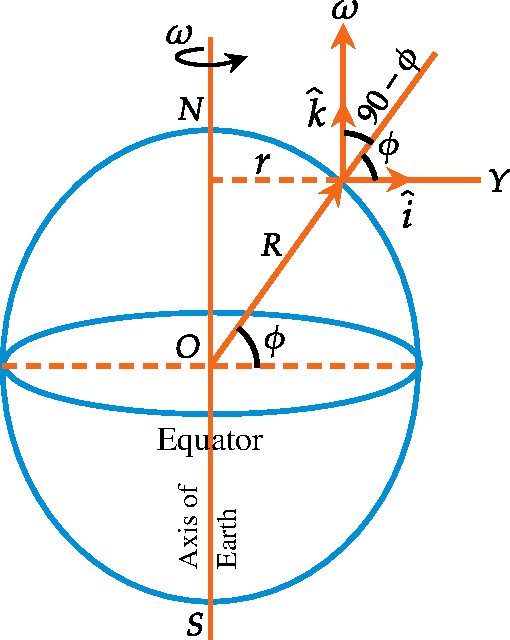
\includegraphics[height=5.5cm,width=5cm]{Centrifugal3}
	\caption{Rotation of earth}
	\label{Rotation of earth}
\end{figure}
\begin{align*}
\text{For earth, $\vec{\omega}$ }&\text{is constant, so,} \\
\frac{d \vec{\omega}}{d t}&=0 \\
\text{Then,}\ \mathrm{a}_{i}&=\mathrm{a}_{r}+2 \vec{\omega} \times \mathrm{v}_{r}+\vec{\omega} \times(\vec{\omega} \times \mathrm{R})\\
\text{If $m$ is the mass of the }&\text{particle, then force in the rotating frame is,}\\
m \mathrm{a}_{r}&=m \mathrm{a}_{i}-2 m \vec{\omega} \times \mathrm{v}_{r}-m \vec{\omega} \times(\vec{\omega} \times \mathrm{R})\\
\text{But,}\ m \mathrm{a}_{r}&=\mathrm{F}_{i}+\mathrm{F}_{0}\\
\text{Therefore fictitious force }&\text{$\mathrm{F}_{0}$ is given by,}\\
\mathrm{F}_{0}&=-2 m \vec{\omega} \times \mathrm{v}_{r}-\vec{\omega} \times(\vec{\omega} \times \mathrm{R})\\
\text{Here $-2 m \vec{\omega} \times \mathrm{v}_{r}$}&\text{ is the Coriolis force and\  $-m \vec{\omega} \times(\vec{\omega} \times \mathrm{R})$, the centrifugal force.}
\end{align*}
\subsection{Azimuthal Force}
Azimuthal Force  appears to act on the particles which are being observed from a rotating frame which has non-uniform angular velocity i.e. $\frac{d \vec{\omega}}{d t} \neq 0$.
It's direction is tangential to the rotation of frame. 
\begin{figure}[H]
	\centering
	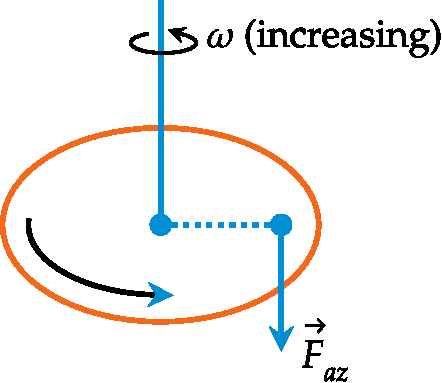
\includegraphics[height=3.8cm,width=4cm]{Azimuthal}
	\caption{Azimuthal force.}
	\label{Azimuthal force}
\end{figure}
\begin{equation}
\text{Azimuthal Force}=-m \frac{d{\vec{\omega}}}{d t} \times r=\vec{F}_{a z}
\end{equation}  
The direction of azimuthal force on a particle lying on a non-uniformly rotating disc is shown in the figure .\ref{Azimuthal force}
\subsection{Centrifugal force}
 The centrifugal force is the only fictitious force, acting on a particle which is at rest $\left(\mathrm{v}_{r}=0\right.$ ) in the rotating frame.  This force goes hand in hand with the ,$ \frac{mv^{2}}{r}=mr\vec{\omega}^{2}$, centripetal acceleration as viewed by someone in an inertial frame. The centrifugal force may be written as, 
\begin{align*}
-m \vec{\omega} \times(\vec{\omega} \times \mathrm{R})&=m \vec{\omega}^{2} \mathrm{r}\\
\text{Where, $r$ is the vector from }&\text{the axis of the earth to the particle and normal to it, because,}\\
\boldsymbol{\vec{\omega}} \times(\boldsymbol{\vec{\omega}} \times \mathrm{R})&=(\boldsymbol{\vec{\omega}} \cdot \mathrm{R}) \vec{\omega}-(\boldsymbol{\vec{\omega}} \cdot \boldsymbol{\vec{\omega}}) \mathrm{R}\\&=\vec{\omega}^{2} R \sin \phi \hat{\mathrm{k}}-\vec{\omega}^{2} R(\hat{\mathrm{i}} \cos \phi+\hat{\mathrm{k}} \sin \phi) \quad[\because \vec{\omega}=\vec{\omega} \hat{\mathrm{k}} \text { and } \mathrm{R}=R(\hat{\mathrm{i}} \cos \phi+\hat{\mathrm{k}} \sin \phi)]\\
&=-\vec{\omega}^{2} R \cos \phi \hat{\mathrm{i}}\\
&=-\vec{\omega}^{2} \mathrm{r} 
\end{align*}
\subsubsection{Effective gravity force ($\mathrm{mg}_{\mathrm{eff}}$).}
 Consider a person standing motionless on the earth, at a polar angle $\theta$. In the rotating frame of the earth, the person feels a centrifugal force (directed away from the axis) in addition to the gravitational force, $m \mathrm{g}$.   Note that we're using $\mathrm{g}$ to denote the acceleration due solely to the gravitational force. 
The sum of the gravitational and centrifugal forces doesn't point radially, unless the person is at the equator or at a pole. Let us denote the sum by $m \mathrm{~g}_{\text {eff }}$. To calculate $m \mathrm{~g}_{\mathrm{eff}}$, we must calculate $\mathrm{F}_{\text {cent }}=$ $-m \vec{\omega} \times(\vec{\omega} \times \mathrm{r})$. The $\vec{\omega} \times \mathrm{r}$ part has magnitude $R \vec{\omega} \sin \theta$, where $R$ is the radius of the earth, and it is directed tangentially along the latitude circle of radius $R \sin \theta$. So $-m \vec{\omega} \times(\vec{\omega} \times \mathrm{r})$ points outward from the axis, with magnitude $m R \vec{\omega}^{2} \sin \theta$, which is just what we expect for something traveling at frequency $\vec{\omega}$ in a circle of radius $R \sin \theta$. Therefore, the effective gravitational force,
$$
m {g}_{\mathrm{eff}} \equiv m({g}-\vec{\omega} \times(\boldsymbol{\vec{\omega}} \times \mathrm{r}))
$$
\begin{center}
\begin{figure}[H]
\begin{minipage}{0.45\textwidth}
	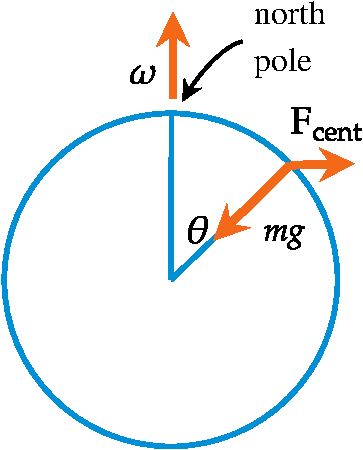
\includegraphics[height=3.6cm,width=3cm]{g-effective 1}
\end{minipage}	\hfil
\begin{minipage}{0.45\textwidth}
	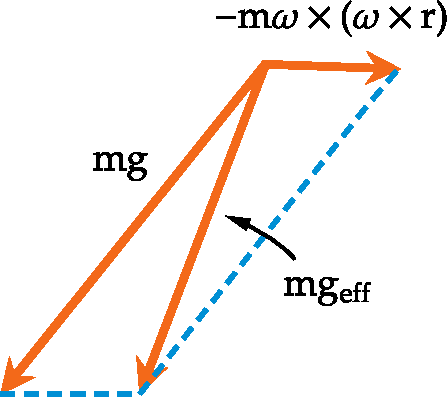
\includegraphics[height=3cm,width=3cm]{g-effective 2}
\end{minipage}	
	\caption{Effective Gravity force}
	\label{Effective Gravity force}
\end{figure}
\end{center}
\subsection{Coriolis force: $-2 m \vec{\omega} \times {v_{r}}$}
Coriolis force is a fictitious force which acts on a particle only  if it is in motion with respect to the rotating frame. In the rotating frame, if a particle moves with velocity $v_{r}$ , then it's always experience a force, ($-2 m \vec{\omega} \times {v_{r}}$) , perpendicular to it's path opposite to the direction of vector product, $\vec{\omega} \times {v_{r}}$.
\begin{figure}[H]
	\centering
	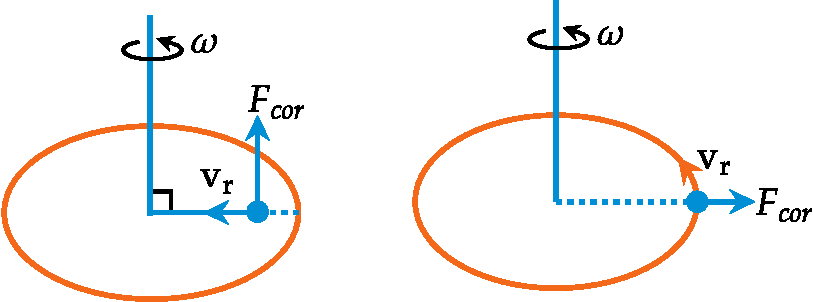
\includegraphics[height=3.5cm,width=7cm]{coriolis}
	\caption{Coriolis force}
	\label{Coriolis force}
\end{figure}
\begin{equation}
\begin{split}
\text{Coriolis force,}\ \vec{F}_{\text {cor }}&=-2 m \vec{\omega} \times \vec{v}_{r}\\  \text{Or}\quad \vec{F}_{c o r}&=2 m \vec{v}_{r} \times \vec{\omega}
\end{split}
\end{equation}\\ The classic Coriolis example is to imagine you are sitting on the north pole and just happen to have a Howizter handy. You fire the thing off and because the earth is turning under the projectile to you the shell is turning to the right. From the point of view of an observer in an inertial frame, the projectile follows a straight path. The angular deflection of the projectile must be $\omega t$, the earth's rotation in time $t$. The effect of coriolis force is appreciable in the condition if it acts horizontal or has a horizontal componet because in the vertical direction it's effect is masked by the large gravitational force.

\begin{abox}
	Practise set-3 
\end{abox}
\begin{enumerate} [label=\color{ocre}\textbf{\arabic*.}]
	\item \textbf{(a)} Given that earth rotates once every $23 \mathrm{~h} 56 \mathrm{~min}$ around the axis from the North to South Pole, calculate the angular velocity, $\omega$, of the earth. When viewed from above the North Pole, the earth rotates counterclockwise (west to east). Which way does $\omega$ point?\\\\
	\textbf{(b)} Foucault's pendulum is a simple pendulum suspended by a long string from a high ceiling. The effect of Coriolis force on the motion of the pendulum is to produce a precession or rotation of the plane of oscillation with time. Find the time for one rotation for the plane of oscillation of the Foucault pendulum at $30^{\circ}$ latitude.
	\begin{answer}
		$ \left. \right.$\\\\
\textbf{(a)}  $\omega$ points in the south to north direction along the rotational axis of the earth.
	\begin{equation*}
\omega=\frac{2 \pi}{T}=\frac{2 \pi}{86,160}=7.292 \times 10^{-5} \mathrm{rad} / \mathrm{s}
	\end{equation*}
\textbf{(b)}The period of rotation of the plane of oscillation is given by
	\begin{equation*}
	T^{\prime}=\frac{2 \pi}{\omega^{\prime}}=\frac{2 \pi}{\omega \sin \lambda}=\frac{T_{0}}{\sin \lambda}=\frac{24}{\sin 30^{\circ}}=48 \mathrm{~h}
	\end{equation*}
\end{answer}


\item An iceberg of mass $5 \times 10^{5}$ tons near the North Pole moves west at the rate of $8 \mathrm{~km} /$ day. Neglecting the curvature of the earth, find the magnitude and direction of the Coriolis force.
\begin{answer}
	\begin{align*}
F_{\text {coriolis }}&=-2 m \omega \times v_{\mathrm{R}} \\
F_{\text {cor }}&=2 m \omega v_{\mathrm{R}} \sin \theta\\&=2 \times 5 \times 10^{8} \times 7.27 \times 10^{-5} \times \frac{8000}{86,400} \quad\left(\because \theta=90^{\circ}\right) \\
&=6730 \mathrm{~N} \text { due north }
	\end{align*}
\end{answer}
\item A train of mass 1000 tons moves in the latitude $60^{\circ}$ north. Find the magnitude and direction of the lateral force that the train exerts on the rails if it moves with a velocity of $15 \mathrm{~m} / \mathrm{s}$.
\begin{answer}
	\begin{align*}
	F_{\text {cor }} &=2 m v \omega \sin \theta \\
	&=2 \times 10^{6} \times 15 \times 7.27 \times 10^{-5} \sin 60^{\circ} \\
	&=1889 \mathrm{~N} \text { on the right rail. }
	\end{align*}
\end{answer}
\item A train of mass $m$ is travelling with a uniform velocity $v$ along a parallel latitude. Show that the difference between the lateral force on the rails when it travels towards east and when it travels towards west is $4 m v \omega \cos \lambda$, where $\lambda$ is latitude and $\omega$ is the angular velocity of the earth.
\begin{answer}
	The difference between the lateral forces on the rails arises because when the train reverses its direction of motion Coriolis force also changes its sign, the magnitude remaining the same. Therefore, the difference between the lateral force on the rails will be equal to $2 m v \omega \cos \lambda-(-2 m v \omega \cos \lambda)$ or $4 m v \omega \cos \lambda$.
\end{answer}
\item  A small block of mass ' $m$ ' lies on a wedge of mass $M$ as shown in figure. All the contact surfaces are smooth. When a horizontal force $\mathrm{F}$ is applied to the wedge, the block does not slide on the wedge. What must be value of $\mathrm{F}$.
\begin{figure}[H]
	\centering
	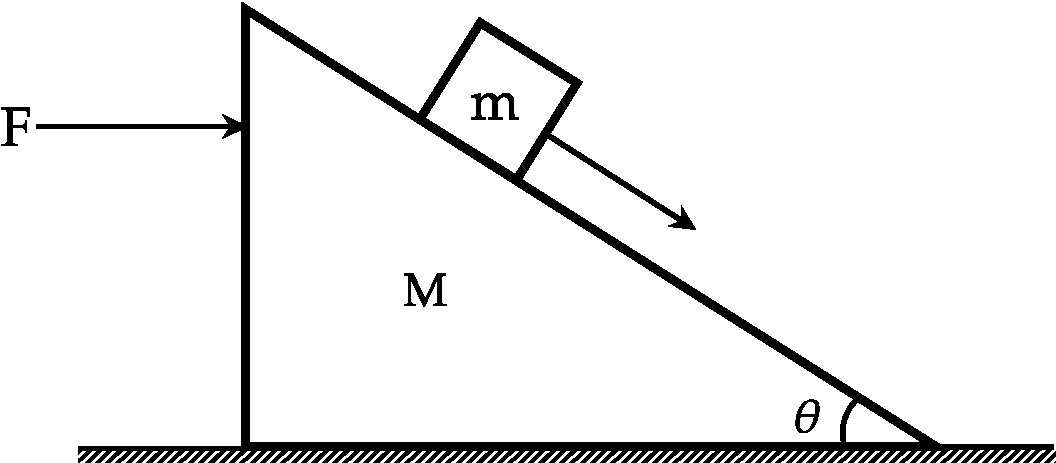
\includegraphics[height=2.2cm,width=5cm]{pset-3- fict}
\end{figure}
\begin{answer}
\begin{align*}
\text { Horizontal acceleration of the system is } a_{0}&=\frac{F}{M+m}
\intertext{According to question, the block does not slide on the wedge, therefore if block is seen from the reference frame of the wedge it will appear stationary. The wedge has a linear acceleration $a_{0}$ therefore if observation is made from the wedge frame a pseudo force $-m a_{0}$ must be applied on the block as shown in figure. Block is stationary on the wedge so component of forces parallel to the inclined plane must cancel.}
\text{Therefore,} \ m g \sin \theta&=m a_{0} \cos \theta\\  \text{or}\ \tan \theta&=\frac{a_{0}}{g}\\&=\frac{F}{(M+m) g}\\ \text{or}\ F&=(M+m) g \tan \theta
\end{align*}
\end{answer}
\item Assuming earth to be a sphere, calculate the linear speed of an object lying on the earth's surface at an altitude of $\lambda=60^{\circ}$ and also calculate the centrifugal force experienced by an object of mass $50 \mathrm{~kg}$. Compare this force with gravitational force.
fictitious pset-3
\begin{answer}
	\begin{align*}
	\text { Angular velocity of earth }&\text{ about its axis due to its spinning motion is}\\
	\omega&=\frac{2 \pi}{T}=\frac{2 \pi}{(24 \times 60 \times 60)} \mathrm{rad} / \mathrm{sec}\\
	\text{At latitude $\lambda=60^{\circ}$ }&\text{objects move in circle of radius $r=R \cos \lambda$}\\
	\therefore \text {Linear speed }&=\omega r\\
	&=\frac{2 \pi}{24 \times 60 \times 60} \times 6400 \times 10^{3} \cos 60^{\circ} \mathrm{m} / \mathrm{s} \\
	&=\frac{2 \pi \times 10^{3}}{27} \mathrm{~m} / \mathrm{s} \quad 233 \mathrm{~m} / \mathrm{s}\\
	\text { Centrifugal force }&=m \omega^{2} r \\
	&=50 \times\left(\frac{2 \pi}{24 \times 60 \times 60}\right)^{2} \times 6400 \times 10^{3} \\
	&\simeq 1.70 \mathrm{~N} \\
	\text { Gravitational force }&=m g=50 \times 9.8\\
	&=490 \mathrm{~N}
	\intertext{Since centrifugal force due to spinning of earth is very small compared to the gravitational force due to this reason we do not feel the rotation of earth.}
	\end{align*}
\end{answer}
\item A person is standing at the edge of a disc of radius $\mathrm{R}$. The dise is rotating about its axis with uniform angular velocity $\omega .$ The person throws a stone in radially outward direction with speed $\frac{\omega R}{2}$ relative for the disc. Calculate acceleration of stone as seen by the person soon after throwing. (neglect gravity).
\begin{answer} $\left. \right. $\\
	\begin{figure}[H]
		\centering
		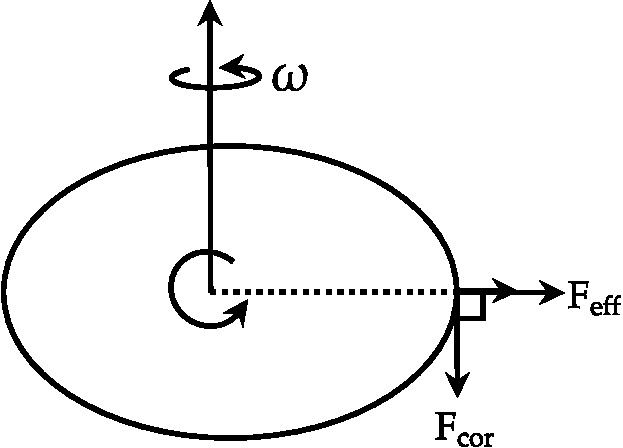
\includegraphics[height=4cm,width=5cm]{fictitious pset-3 1}
	\end{figure}
	\begin{align*}
	\intertext{As seen by the person the stone is acted upon by centrifugal and coriolis forces. The direction of the two forces soon after throwing is shown in the figure. Net force on the stone is}
	F^{\prime}&=\sqrt{F_{c o r}^{2}+F_{c f}^{2}} \\
	&=\sqrt{\left|2 m \vec{v}^{\prime} \times \vec{\omega}\right|^{2}+\left(m \omega^{2} r_{\perp}\right)^{2}}\\&=\sqrt{\left(2 m \frac{\omega R}{2} \omega \sin 90^{\circ}\right)^{2}+ (m \omega^{2}R )^{2}} \\
	F^{\prime}&=\sqrt{2} m \omega^{2} \\
	\text{Then the }&\text{acceleration,}\\
	a^{\prime}&=\frac{F^{\prime}}{m}=\sqrt{2} \omega^{2} R
	\end{align*}
\end{answer}
\end{enumerate}